One of the major performance metrics of interest to end-users, is the application's completion time. 
To evaluate this, we develop an analytical model for the expected completion time of Lazy Shadowing, with all probabilities of failures considered. We assume that failures don't happen at the same time.
%Since we are comparing between Lazy Shadowing and process replication, the overhead of failure detection and consistency protocols are ignored as they are the same for the two approaches.
%Our models focus on one 
%checkpointing interval of the application, since the whole execution is just a repetition of multiple such intervals. As a consequence, we assume the execution with checkpointing starts right after the previous checkpoint and ends right before the next checkpoint, and the execution with Lazy Shadowing and process replication will not experience any application failure. For fairness, we assume that the three alternatives have the same amount of workload, 
%$W$, to execute, and total number of available cores, $M$. The maximal execution rate at each core, $\sigma_{max}$, is normalized to 1 so that the time to complete without failures is equal to the workload to execute on each core. In addition, we assume that the three alternatives will encounter the same number of failures, which is $k$, as they will execute the same amount of workload using the same amount of resources.

%\subsubsection{Expected completion time}
First we discuss the case of $k$ failures, which separate the execution into $k+1$ intervals.
Denote by $\Delta_i$ ($1\le i \le k+1$) the $i^{th}$ continuous execution interval, and $\tau_i$ ($1\le i \le k$) the recovery time after $\Delta_i$. 
%between the $(i-1)^{th}$ and $i^{th}$ failures (assuming the $0^{th}$ failure happens right before the execution begins, and the $(k+1)^{th}$ failure happens right after the execution ends), and $\tau_i$ ($1\le i \le k$) the recovery time after the $i^{th}$ failure. 
The application's progress with delay incurred by failures is illustrated in Figure~\ref{fig:progress}.

\begin{figure}[!t]
	\begin{center}
		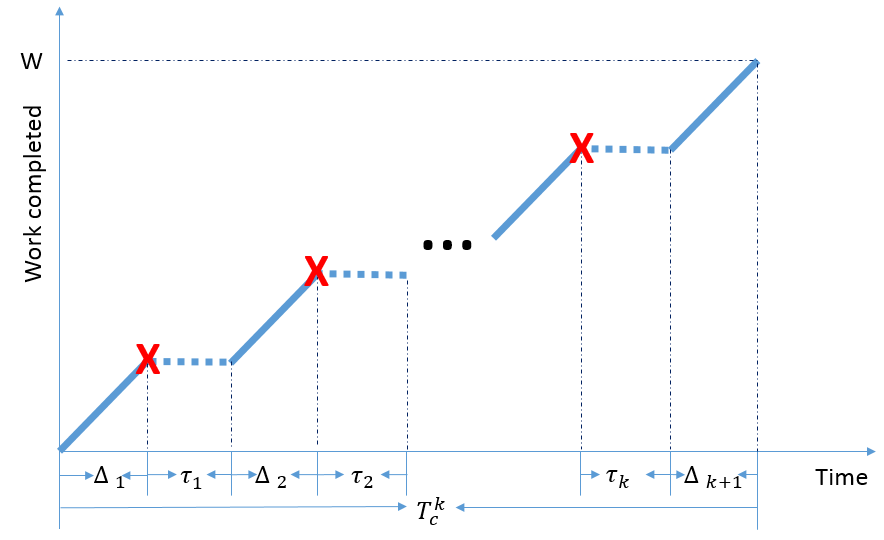
\includegraphics[width=\columnwidth]{Figures/progress}
	\end{center}
	%\vskip -0.22in 
	\caption{Illustration of application's progress with failure incurred delays.}
	\label{fig:progress}
\end{figure}

Since Lazy Shadowing use $M$ cores for executing main processes and $S$ cores for shadowing ($M+S=N$), the total workload $W$ will be split into $M$ tasks, each of which will be assigned a pair of main and shadow processes. Therefore, the workload of each process is 
$w=W/M$. The recovery time $\tau_i$ is the time needed for the lazy shadow of the failed main to catch up. With shadow leaping, it is guaranteed that all the shadows reach the same execution point as the mains (See Figure~\ref{fig:leap}) after the previous recovery, so every recovery time is proportional to its previous continuous execution length, which is $\Delta_i$. That is, $\tau_i = \Delta_i \times (1 - \sigma_s^b)$. The value of $\Delta_i$ can be obtained given a failure probability distribution, as will be demonstrated in Section~\ref{sec:evaluation}. 
Since we assume there are $k$ failures, then $\Delta_{k+1}$ is the failure free execution interval until $W$ is complete, i.e., $\Delta_{k+1} = w - \sum_{i=1}^{k}\Delta_i$. Finally, according to Figure~\ref{fig:progress}, the completion time with $k$ failures is 
\begin{equation}
	T_c^k = \sum_{i=1}^{k+1}\Delta_i + \sum_{i=1}^k\tau_i = w + (1-\sigma_s^b)\sum_{i=1}^k\Delta_i
	\label{eq:time_k}
\end{equation}

We assume that failures do not occur during recovery, so the failure probability of a core during the execution can be estimated as $P_c = F(w)$. Then the probability that there are $k$ failures among the $N$ cores during the execution is 
\begin{equation}
\begin{split}
P_s^{k}= & \dbinom{N}{k}{P_c}^k(1-P_c)^{N-k} \\
%= & \dbinom{M}{k}({\frac{w}{MTTI}})^k(1-\frac{w}{MTTI})^{M-k}
\end{split}
\end{equation}

The completion time considering all possible failures can be averaged as $T_{c} = \sum_{i} T_{c}^{i} \cdot P_s^{i}$, and the expected completion time considering the possibility of re-execution after application failure is
%\begin{equation} 
%E[T_{c}] = \sum_{i} T_{c}^{i} \cdot P_s^{i}
%\label{eq:exp_time}
%\end{equation}
\begin{equation} 
T_{total} = T_{c} / (1 - P_a)
\label{eq:exp_time}
\end{equation}

In the special case of $\alpha=1$, which is process replication, half of the hardware resources are dedicated to replicas so that the workload assigned to each task is significantly increased given the fixed number of cores available, i.e., $w=2W/N$. Different from the case of $\alpha \ge 2$, failures do not incur any delay unless application failure occurs, since the replicas are executing at the same rate as the main processes. Therefore, the completion time of process replication without application failure is constant with respect to the number of failures, and the expected completion time considering the possibility of re-execution is
\begin{equation}
	T_{total} = T_c / (1 - P_a) = w / (1 - P_a)
\end{equation}

A closer look at the above analysis one can realize that Lazy Shadowing has both advantage and disadvantage compared to traditional process replication. When collocating multiple shadow processes on each core, more resources will be dedicated to main processes, leading to less workload per process and thus less completion time. On the other hand, however, collocation slows down the shadow processes, implying delays when failures occur. Although it may seem that the delay would keep deteriorating as the number of failures increases, it turns out to be well bounded, as a result of shadow leaping. From Equation~\ref{eq:time_k} we can see the delay of $k$ failures is $(1-\sigma_s^b)\sum_{i=1}^k\Delta_i$. Since we have the relation $\Delta_{k+1} = w - \sum_{i=1}^{k}\Delta_i$, $\sum_{i=1}^{k}\Delta_i$ is bounded by $w$, effectively limiting the delay by $(1-\sigma_s^b)w$.

%Contrary to process replication and Lazy Shadowing, checkpointing can use all the available cores to share the total workload, so that $w = W/M$. However, the drawback is that each failure would result in an application failure which needs to roll back the execution to the last checkpoint. With that said, the recovery time of each failure is equal to the normal execution time from the last checkpoint to the time of the failure, i.e., $\tau_i = \sum_{j=1}^{i}\Delta_j$. The completion time with $k$ failures is $T_c^k = \sum_{i=1}^{k+1}\Delta_i + \sum_{i=1}^k\tau_i = w + \sum_{i=1}^{k}\sum_{j=1}^i\Delta_j$.

%\subsubsection{Expected energy consumption}





